\documentclass[12pt]{article} % Default font size is 12pt, it can be changed here

\usepackage[utf8]{inputenc} % utf8 encoding
\usepackage{geometry} % Required to change the page size to A4
\geometry{a4paper} % Set the page size to be A4 as opposed to the default US Letter

\usepackage{graphicx} % Required for including pictures
\usepackage{amsmath}
\usepackage{float} % Allows putting an [H] in \begin{figure} to specify the exact location of the figure

\linespread{1.2} % Line spacing

%\setlength\parindent{0pt} % Uncomment to remove all indentation from paragraphs

\graphicspath{{pictures/}} % Specifies the directory where pictures are stored

\usepackage{listings} % To be able to have code in text
\usepackage{color} % To be able to have colors

\definecolor{codegreen}{rgb}{0,0.6,0}
\definecolor{codegray}{rgb}{0.5,0.5,0.5}
\definecolor{codepurple}{rgb}{0.58,0,0.82}
\definecolor{backcolour}{rgb}{0.95,0.95,0.92}
 
\lstdefinestyle{codestyle}{
    backgroundcolor=\color{backcolour},   
    commentstyle=\color{codegreen},
    keywordstyle=\color{magenta},
    numberstyle=\tiny\color{codegray},
    stringstyle=\color{codepurple},
    basicstyle=\footnotesize,
    breakatwhitespace=false,         
    breaklines=true,                 
    captionpos=b,                    
    keepspaces=true,                 
    numbers=left,                    
    numbersep=5pt,                  
    showspaces=false,                
    showstringspaces=false,
    showtabs=false,                  
    tabsize=2
}
 
\lstset{style=codestyle}

\begin{document}

%----------------------------------------------------------------------------------------
%   TITLE PAGE
%----------------------------------------------------------------------------------------

\begin{titlepage}

\newcommand{\HRule}{\rule{\linewidth}{0.5mm}} % Defines a new command for the horizontal lines, change thickness here

\center % Center everything on the page

\textsc{\LARGE Lund University, Faculty of Engineering}\\[1.5cm] % Name of your university/college
\textsc{\Large ETIA10}\\[0.5cm] % Major heading such as course name
\textsc{\large Patent and Intellectual Property Rights}\\[0.5cm] % Minor heading such as course title

\HRule \\[1cm]
{ \huge \bfseries Summary of ETIA10}\\[0.4cm] % Title of your document
\HRule \\[1.5cm]

\emph{Author:} Fred \textsc{Nordell} % Your name

{\large \today}\\[3cm] % Date, change the \today to a set date if you want to be precise

%\includegraphics{Logo}\\[1cm] % Include a department/university logo - this will require the graphicx package

\vfill % Fill the rest of the page with whitespace

\end{titlepage}

%----------------------------------------------------------------------------------------
%   TABLE OF CONTENTS
%----------------------------------------------------------------------------------------

\tableofcontents % Include a table of contents
\lstlistoflistings % Include a table of lstlistings
\listoffigures % Include listing of figures
\listoftables % Include listing of tables

\newpage % Begins the essay on a new page instead of on the same page as the table of contents 


\section{Introduction} % Major section


\section{General IPR}


Intelectual property right refers to (astract) products of the human intellect that have a (commercial) value and that may recieve legal protection.


Different type of IP laws:

\begin{itemize}
   \item Patent law
   \item Copyright law
   \item Trademark law
   \item Design rights
   \item Trade secret laws 
\end{itemize}


\section{Patent}

Rights conferred bt the patent

\begin{itemize}
    \item Prevent othters from making, using, offering fro sale, selling or importing infringin products 
    \item Right to assign or transfer ownership
    \item Lasts for up to 20 years after filing
\end{itemize}


Rights NOT conferred by the patent

\begin{itemize}
    \item Does not grant right to make, use offer for sale of import the invention. Only exclude others.
    \item Since the patent does not grant the right to make, use, offer for sale, or sell, or import the invention, the patentee’s own right to do so is dependent upon the rights of others and whatever general laws might be applicable.
    \item Does not guarantee commercial success.
    \item Purpouse is not to establish long-monopolies. hey are granted for a limited period, which can only be extended in the case of medicines and pesticides which have to undergo lengthy clinical trials for safety reasons.
\end{itemize}

A patent must solve a \textbf{technical problem} and be \textit{new}, \textit{inventive} - not an ``obvious'' solution, \textit{susceptible of industrial application}.

\subsection{Application process}

There are three ways to apply:
\begin{enumerate}
    \item National application
    \item Regional application (e.g. EPC)
    \item International (IPC)
\end{enumerate}

Note however that there is \textbf{no such thing} as a \textit{World patent}, but only a international application.

Things consider before an application:

\begin{itemize}
    \item No publication prior to filing
    \item No sale of products with the invention
    \item No lecture or presentaation, exept under NDA
    \item Seek professional advice ASAP
\end{itemize}

\subsubsection{EPC}

The Convention on the Grant of European Patents (5\textsuperscript{th} Oct. 1973), commonly known as the European Patent Convention (EPC), is a multilateral treaty instituting the European Patent Organisationand providing an autonomous legal system according to which European patents are granted.

It is a way to file a single application for all 38 contracting states and 2 extention states through the same procedure.

\paragraph{Regional route}

\begin{itemize}
    \item one application filed at one office for all 40 states
    \item one procedure
    \item applicants select states
    \item results in a bundle of national patents
    \item one European patent for up to 40 states
\end{itemize}

\paragraph{What the EPC is}

\begin{itemize}
    \item 178 Articles
    \item 165 Rules
    \item Misc. additional rules, Case law and guidelines
\end{itemize}

Important Articles, Rules and Guidelines:
\begin{itemize}
    \item Article 2 \& 3: Foundational
    \item 52: Patentable inventions
    \item 53 \& Rule 28, 29: Exceptions to patentability 
    \item 54 \& 55: Novelty
    \item 56: Inventive step
    \item 57: Industrial aplication
    \item 58 \& 59: Who can file a patent
    \item 69: Extent of protection
    \item Guideline 11.3: Person skilled in the arts
\end{itemize}

State of the art, or Prior art, is \textit{any evidence that your invention is already known}.
And this only has to be that someone, somewhere has described what you claim to have invented.
\textbf{Anything} can be prior art, however secret information might not be. provied that those with access are under an NDA.

\paragraph{EPC filing process, Lecture 4}

\begin{figure}[]
    \centering
    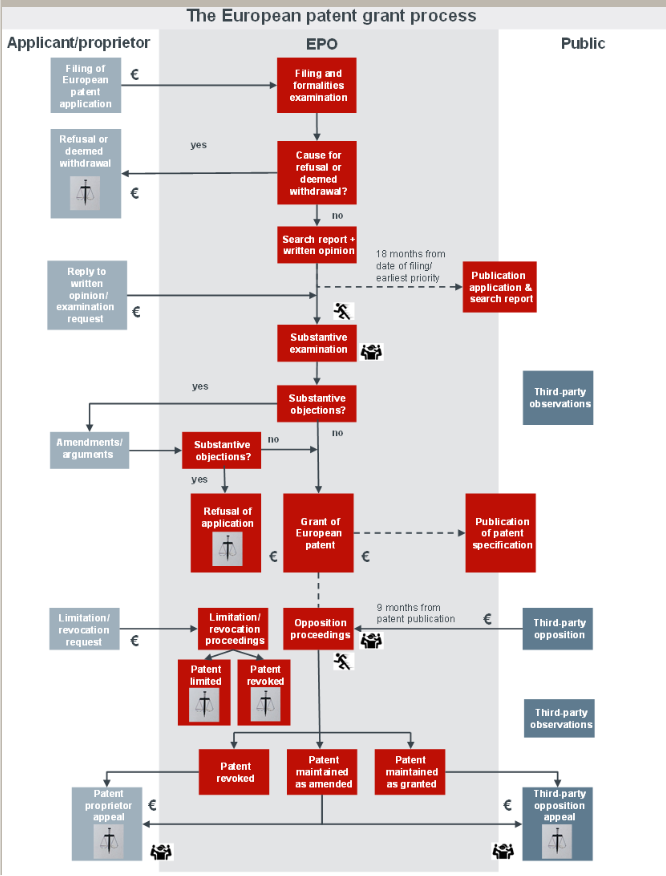
\includegraphics[]{EPC_process.png}
    \caption{EPC filing process}
    \label{fig:EPC_process}
\end{figure}


\textit{Date of filiing}: You can request a date of filing wothout clamis.
However, that gives you a two month period in wich you have to provide a claim.
Relevant articles are: 80, 75, 78

\par \textit{Fees}: Relevant articles: 51

\par \textit{Requirements}: Relevant articles: 83, 84, 85

\par A search is carried out by an examiner at the EPO. It will result in a European search report + Written Opinion.
Relevant rules: 61, 71.
After this step the appolication is publised, normally with teh search report. 18 months after filiing date or priority date!
Strategic descision time: Should you go forward of withdraw.
Relevant article: 93
After this you have six months to decide.

\par \textit{Request for examination}: Rule 70.
In the sustansive examination Third parties can do obsevations, and influence the outcome!
Article 115!


\par \textit{Grant step}: You might have to translate as the grant is for a bundle of national patents. The specification should be published ASAP in the Patent Bulletin.
Article: 97, 98, 63, 64, 67, 60
Patents are only enforable from grant period. Opposition is possible, must be filed within 9 months.


\subsection{PCT - Patent Cooperation treaty, Lecture 5}
Treaty concluden in 1970, basically the EPC but international.
Word Intellectual property Organisation manages some tasks, is part of UN.

\par Consists of 69 articles, 96 rules and a number of guidelines and case law.

\textbf{A PCT will not result in a International patent!} It is in the same way EPC is, a pplication route.

\begin{figure}[H]
    \centering
    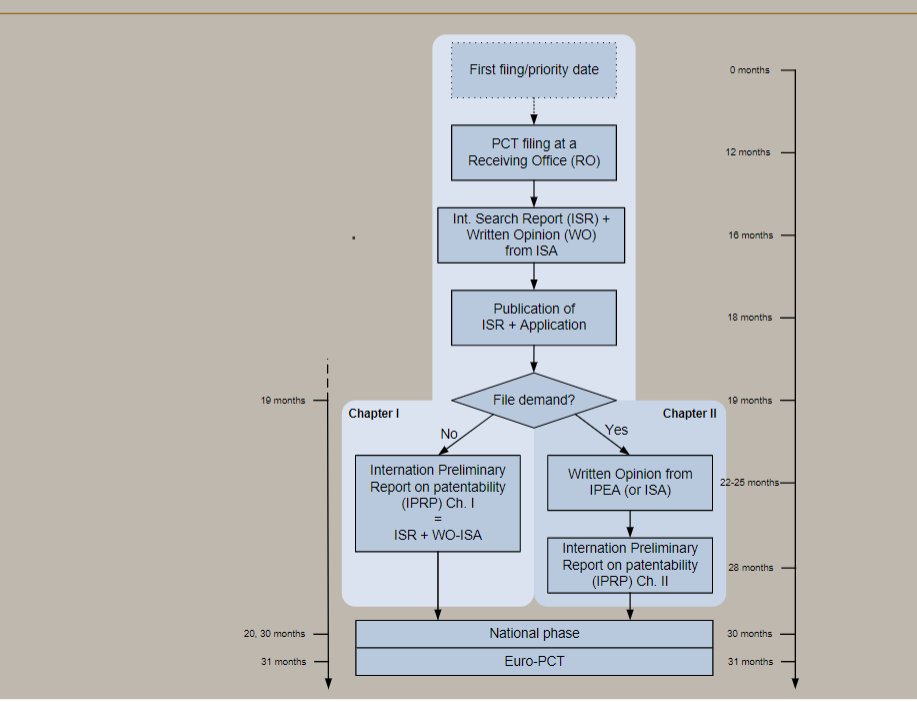
\includegraphics[width=\textwidth]{TCP_process.png} 
    \caption{TCP track}
    \label{fig:tcp_process}
\end{figure}

Can be filed in multiple languages, but you might have to furnish a translation


\subsection{UMP}
A utility model is a statutory monopoly granted for a limited time in exchange for an inventor providing sufficient teaching of his or her invention to permit a person of ordinary skill in the relevant art to perform the invention. 

\par It is basically a small patent, ostly used to get incremential invention patents.

Differences:
\begin{itemize}
    \item Requirements are lesser.
    \item shorter rights, betweent 7 to 10 years
    \item shorter process
    \item cheaper
    \item might be restricted to certain fields
    \item primarily used for mechanical inventions
\end{itemize}



\section{Desing and trademark}

\subsection{Design}

The Design has to be new, this is regualted in article 5.
The individuallity is assed mostly on the overall impression of the product.

\par In essence: The lower the degree of freedom in developing the Design (e.g. due to technical reasons; a table needs four legs / consumer expectations; a mobile phone has a display and keypad), the lower the requirements for what constitutes Individual Character

\begin{figure}[H]
    \centering
    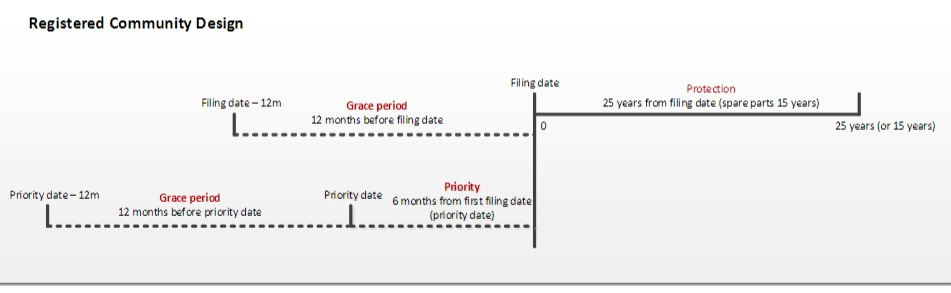
\includegraphics[width=\textwidth]{design.jpg}
    \caption{Design process}
    \label{fig:design}
\end{figure}

\subsection{Trademark}

A trademark is any mark, sign or indication that is used for indicating goods or services in commerce. 

Must be distinctive.

\begin{figure}[]
    \centering
    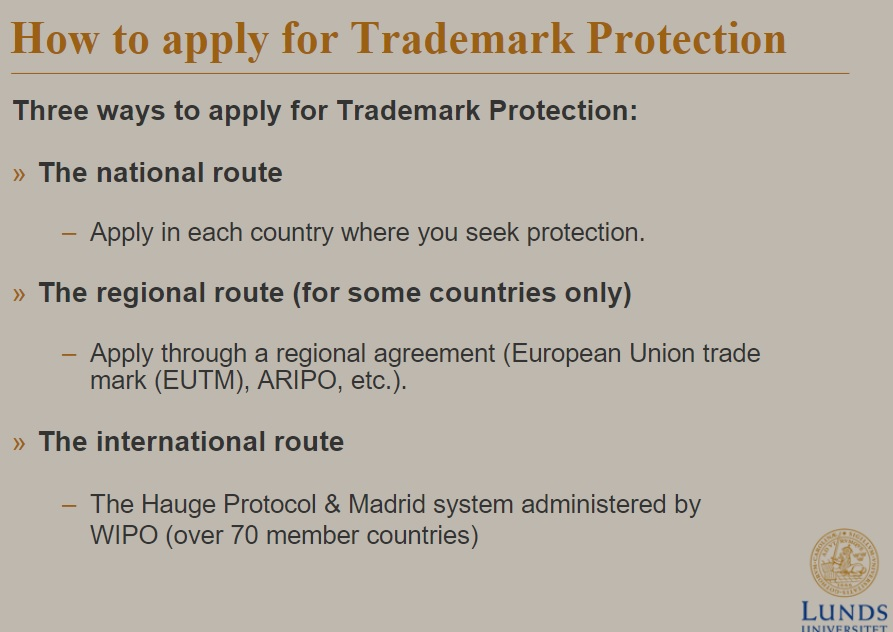
\includegraphics[width=\textwidth]{trademark.jpg}
    \caption{Routes for trademark protection}
    \label{fig:trademark}
\end{figure}


\section{Geographical indications}

Is valauble because it will certify that a product is from somewhare and that can be used for marketing and or take a larger margin!
There are some international agreements about this. In the US this is a kind of trademark.

e.g. Champange

\section{Copyright}

A right to benefit financially from the work is articulated, and court rulings and legislation have recognized a right to control the work, such as ensuring that the integrity of it is preserved. 

\par If you can se, hear and/or touch the work it is protected under copyright.


Economic rigth - Usually transferable:
\begin{itemize}
    \item Reproduction: right to make copies of the work in any manner or form.
    \item Communiaion ot the public: transmition, publiv performance et.
    \item Adaptation, translation etc.
\end{itemize}

Moral rights - usually not transferable:
\begin{itemize}
    \item Parternity: right to be mentioned as author
    \item integrity: right to object to mutilation, distortion etc.
\end{itemize}

The length is often authors life + 50 or 70 years.

\end{document}